\documentclass{article}
\usepackage{graphicx}
\usepackage[nomarkers]{endfloat}
\begin{document}

\begin{figure}

\includegraphics{fig_test}
\caption{Figure test using includegraphics.} 
\label{figure1}
\end{figure}

Figure \ref{figure1} tests \verb#\epsffile{fig_test.eps}#.
filler filler filler filler filler filler filler filler filler
filler filler filler filler filler filler filler filler filler
filler filler filler filler filler filler filler filler filler
filler filler filler filler filler filler filler filler filler
filler filler filler filler filler filler filler filler filler
filler filler filler filler filler filler filler filler filler
filler filler filler filler filler filler filler filler filler
filler filler filler filler filler filler filler filler filler
filler filler filler filler filler filler filler filler filler
filler filler filler filler filler filler filler filler filler
filler filler filler filler filler filler filler filler filler
filler filler filler filler filler filler filler filler filler
filler filler filler filler filler filler filler filler filler
filler filler filler filler filler filler filler filler filler
filler filler filler filler filler filler filler filler filler
filler filler filler filler filler filler filler filler filler
filler filler filler filler filler filler filler filler filler
filler filler filler filler filler filler filler filler filler
filler filler filler filler filler filler filler filler filler
filler filler filler filler filler filler filler filler filler
filler filler filler filler filler filler filler filler filler
filler filler filler filler filler filler filler filler filler
filler filler filler filler filler filler filler filler filler
filler filler filler filler filler filler filler filler filler
filler filler filler filler filler filler filler filler filler
filler filler filler filler filler filler filler filler filler
filler filler filler filler filler filler filler filler filler
filler filler filler filler filler filler filler filler filler
filler filler filler filler filler filler filler filler filler
filler filler filler filler filler filler filler filler filler

\begin{figure*}

\includegraphics[width=4in]{fig_testa}
\caption{Figure* test using includegraphics.} 
\label{figure1a}
\end{figure*}

\begin{table}
\begin{center}
\begin{tabular}{llr}
\multicolumn{2}{c}{Item} & \multicolumn{1}{c}{Price} \\
gnat      & (dozen)  & 3.24\\
gnu       & (each)   & 24,985.47 
\end{tabular}
\caption{Simple example from the \LaTeX{} manual exhibiting multicolumn.}
\end{center}
\end{table}

Figure \ref{figure1} tests \verb#\epsffile{fig_test.eps}#.
filler filler filler filler filler filler filler filler filler
filler filler filler filler filler filler filler filler filler
filler filler filler filler filler filler filler filler filler
filler filler filler filler filler filler filler filler filler
filler filler filler filler filler filler filler filler filler
filler filler filler filler filler filler filler filler filler
filler filler filler filler filler filler filler filler filler
filler filler filler filler filler filler filler filler filler
filler filler filler filler filler filler filler filler filler
filler filler filler filler filler filler filler filler filler
filler filler filler filler filler filler filler filler filler
filler filler filler filler filler filler filler filler filler
filler filler filler filler filler filler filler filler filler
filler filler filler filler filler filler filler filler filler
filler filler filler filler filler filler filler filler filler
filler filler filler filler filler filler filler filler filler
filler filler filler filler filler filler filler filler filler
filler filler filler filler filler filler filler filler filler
filler filler filler filler filler filler filler filler filler
filler filler filler filler filler filler filler filler filler
filler filler filler filler filler filler filler filler filler
filler filler filler filler filler filler filler filler filler
filler filler filler filler filler filler filler filler filler
filler filler filler filler filler filler filler filler filler
filler filler filler filler filler filler filler filler filler
filler filler filler filler filler filler filler filler filler
filler filler filler filler filler filler filler filler filler
filler filler filler filler filler filler filler filler filler
filler filler filler filler filler filler filler filler filler
filler filler filler filler filler filler filler filler filler

\begin{figure}
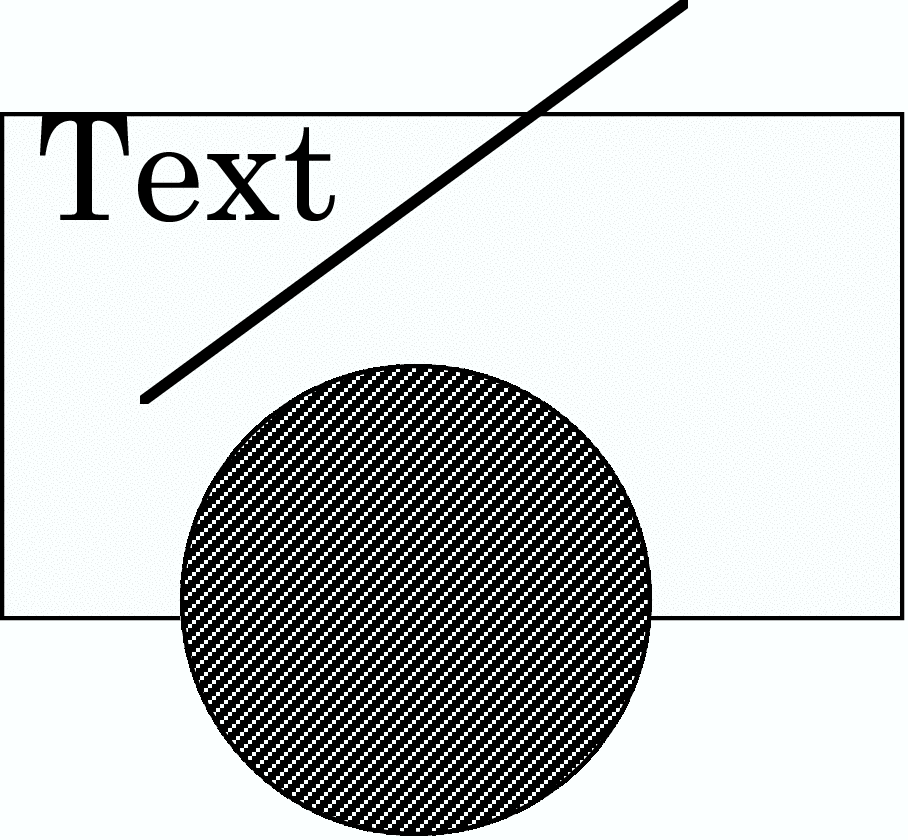
\includegraphics{fig_testb}
\caption{Another Figure test using includegraphics.} 
\label{figure2}
\end{figure}

Figure \ref{figure2} tests \verb#\includegraphic{fig_test.eps}#.
filler filler filler filler filler filler filler filler filler
filler filler filler filler filler filler filler filler filler
filler filler filler filler filler filler filler filler filler
filler filler filler filler filler filler filler filler filler
filler filler filler filler filler filler filler filler filler
filler filler filler filler filler filler filler filler filler
filler filler filler filler filler filler filler filler filler
filler filler filler filler filler filler filler filler filler
filler filler filler filler filler filler filler filler filler
filler filler filler filler filler filler filler filler filler
filler filler filler filler filler filler filler filler filler
filler filler filler filler filler filler filler filler filler
filler filler filler filler filler filler filler filler filler
filler filler filler filler filler filler filler filler filler
filler filler filler filler filler filler filler filler filler
filler filler filler filler filler filler filler filler filler
filler filler filler filler filler filler filler filler filler
filler filler filler filler filler filler filler filler filler
filler filler filler filler filler filler filler filler filler
filler filler filler filler filler filler filler filler filler
filler filler filler filler filler filler filler filler filler
filler filler filler filler filler filler filler filler filler
filler filler filler filler filler filler filler filler filler
filler filler filler filler filler filler filler filler filler
filler filler filler filler filler filler filler filler filler
filler filler filler filler filler filler filler filler filler
filler filler filler filler filler filler filler filler filler
filler filler filler filler filler filler filler filler filler
filler filler filler filler filler filler filler filler filler
filler filler filler filler filler filler filler filler filler

\begin{figure}
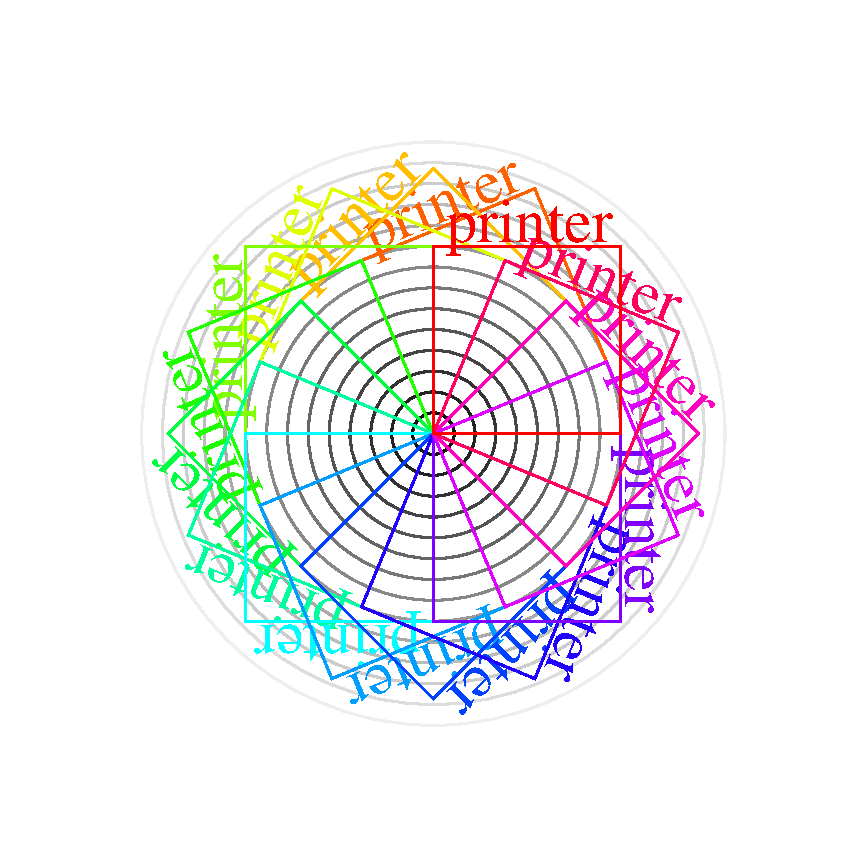
\includegraphics{fig_testc}
\caption{Another Figure test using includegraphics.} 
\label{figure3}
\end{figure}


\begin{table}
\begin{center}
\begin{tabular}{||l|lr||}
\hline
gnats     & gram    & \$13.65 \\
\hline
          & each    &     .01 \\
\hline
gnu       & stuffed &   92.50 \\
\cline{1-1} \cline{3-3}
emur      &         &   33.33 \\
armadillo & frozen  &    8.99 \\
\hline
\end{tabular}
\caption{Simple example from the \LaTeX{} manual exhibiting horizontal
and vertical lines.}
\end{center}
\end{table}


Figure \ref{figure3} tests \verb#\psfig{figure=fig_test.eps}#.
filler filler filler filler filler filler filler filler filler
filler filler filler filler filler filler filler filler filler
filler filler filler filler filler filler filler filler filler
filler filler filler filler filler filler filler filler filler
filler filler filler filler filler filler filler filler filler
filler filler filler filler filler filler filler filler filler
filler filler filler filler filler filler filler filler filler
filler filler filler filler filler filler filler filler filler
filler filler filler filler filler filler filler filler filler
filler filler filler filler filler filler filler filler filler
filler filler filler filler filler filler filler filler filler
filler filler filler filler filler filler filler filler filler
filler filler filler filler filler filler filler filler filler
filler filler filler filler filler filler filler filler filler
filler filler filler filler filler filler filler filler filler
filler filler filler filler filler filler filler filler filler
filler filler filler filler filler filler filler filler filler
filler filler filler filler filler filler filler filler filler
filler filler filler filler filler filler filler filler filler
filler filler filler filler filler filler filler filler filler
filler filler filler filler filler filler filler filler filler
filler filler filler filler filler filler filler filler filler
filler filler filler filler filler filler filler filler filler
filler filler filler filler filler filler filler filler filler
filler filler filler filler filler filler filler filler filler
filler filler filler filler filler filler filler filler filler
filler filler filler filler filler filler filler filler filler
filler filler filler filler filler filler filler filler filler
filler filler filler filler filler filler filler filler filler
filler filler filler filler filler filler filler filler filler

\begin{figure}

\includegraphics{fig_testd}
\caption{Yet another Figure test using includegraphics.} 
\label{figure4}
\end{figure}

Figure  \ref{figure4} tests \verb#\includegraphic{fig_testc.ps}#.  

\end{document}
